\documentclass[conference,a4paper]{IEEEtran}
\usepackage[T1]{fontenc}
\usepackage{amsmath,amssymb,amsthm}
\usepackage{booktabs}
\usepackage{array}
\usepackage{url}
\usepackage{cite}
\usepackage{pgfplots}
\usetikzlibrary{positioning,arrows.meta,shapes.geometric}
\pgfplotsset{compat=1.17}
\brokenpenalty=10000
\newcommand{\FNfoneZero}{0.309}
\newcommand{\FNfoneOne}{0.672}
\newcommand{\FNfoneOAOne}{0.408}
\newcommand{\FNconfOne}{0.302}
\newcommand{\phatThree}{0.384}
\newcommand{\PowESVZero}{0.280}
\newcommand{\PowESVHalf}{0.141}
\newcommand{\PowESVWorst}{0.052}
\newcommand{\PowOAHalf}{0.204}
\newcommand{\PowOAWorst}{0.150}
\newcommand{\ExtCalls}{30\%}
\newcommand{\Nquestions}{1,109}
\newcommand{\NholdClosed}{188}
\newcommand{\SEhold}{0.022}
\newcommand{\HoldNse}{1.2}
\newcommand{\Nscores}{twelve}
\newcommand{\NconfViolOne}{ten}
\newcommand{\ConfAllBy}{0.3}
\newcommand{\MaxInsitu}{0.101}
\newcommand{\MaxTransfer}{0.100}
\newcommand{\FNbgeZero}{0.236}
\newcommand{\FNbgeOne}{0.731}
\newcommand{\PowBGEZero}{0.443}
\newcommand{\PowBGEHalf}{0.173}
\newcommand{\PowBGEOne}{0.097}
\newcommand{\RobPMEsvIn}{0.099}
\newcommand{\RobPMEsvTr}{0.094}
\newcommand{\RobPMAllIn}{0.101}
\newcommand{\RobPMAllTr}{0.100}
\newcommand{\RobPMConf}{0.302}
\newcommand{\RobPTEsvIn}{0.099}
\newcommand{\RobPTEsvTr}{0.094}
\newcommand{\RobPTAllIn}{0.101}
\newcommand{\RobPTAllTr}{0.104}
\newcommand{\RobPTConf}{0.277}
\newcommand{\RobHMEsvIn}{0.117}
\newcommand{\RobHMEsvTr}{0.104}
\newcommand{\RobHMAllIn}{0.126}
\newcommand{\RobHMAllTr}{0.126}
\newcommand{\RobHMConf}{0.299}
\newcommand{\RobHTEsvIn}{0.115}
\newcommand{\RobHTEsvTr}{0.108}
\newcommand{\RobHTAllIn}{0.125}
\newcommand{\RobHTAllTr}{0.125}
\newcommand{\RobHTConf}{0.279}
\newcommand{\ClimN}{1,381}
\newcommand{\ClimFoneMax}{0.60}
\newcommand{\ClimFoneZeroMin}{0.29}
\newcommand{\ClimFoneZeroMax}{0.42}
\newcommand{\ClimConfMax}{0.240}
\newcommand{\ClimCertMax}{0.103}
\newcommand{\ClimDensePowZero}{0.256}
\newcommand{\ClimDensePowOne}{0.195}
\newcommand{\RetroY}{2010}
\newcommand{\RetroYears}{2008, 2010 and 2012}
\newcommand{\RetroNclosed}{310}
\newcommand{\RetroNfilled}{326}
\newcommand{\RetroNnei}{416}
\newcommand{\RetroVisible}{56\%}
\newcommand{\RetroBestPow}{68\%}
\newcommand{\RetroBestPrec}{96\%}
\newcommand{\RetroMaxFN}{0.102}
\newcommand{\RetroFoneMin}{28\%}
\newcommand{\RetroFoneMax}{40\%}
\newcommand{\RetroNdossier}{139}
\newcommand{\RetroLag}{4}
\newcommand{\LLMfone}{0.629}
\newcommand{\LLMfn}{0.378}
\newcommand{\LLMaucFull}{0.687}
\newcommand{\LLMaucDel}{0.477}
\newcommand{\LLMfoneOne}{0.617}
\newcommand{\LLMpowZero}{0.191}


\newtheorem{theorem}{Theorem}
\newtheorem{corollary}{Corollary}
\theoremstyle{definition}
\newtheorem{definition}{Definition}

\newcommand{\open}{\textup{\textsc{open}}}
\newcommand{\closed}{\textup{\textsc{closed}}}

\title{Absence of Evidence Is Not a Research Gap:\\Certified Gap Claims under Corpus Incompleteness}

\author{\IEEEauthorblockN{Anh Hoa Le, Ly Van Khoa Phan, Dinh Thanh Nguyen, Duc Hoang Nguyen, Dinh Anh Ho, Long Truong}
\IEEEauthorblockA{FPT University, Vietnam\\
leanhhoa30012004@gmail.com, khoaplvse181656@fpt.edu.vn, thanhndse182854@fpt.edu.vn,\\
hoangndse181655@fpt.edu.vn, anhhdse180670@fpt.edu.vn, longt5@fpt.edu.vn}}

\begin{document}
\maketitle

\begin{abstract}
Tools that propose research gaps usually treat a question as open when their corpus holds no paper that answers it. That inference fails whenever the corpus is incomplete, which is the normal case. We study gap claims as a decision problem with a measurable error: declaring a question \open{} although the literature already answers it (false novelty). We build GapClose-SciFact, a benchmark of 1,109 questions derived from expert-annotated SciFact claims, and simulate missing literature by deleting gold evidence documents. Thresholds tuned for accuracy call 20\% to 32\% of answered questions open on a complete corpus and up to 73\% when evidence is missing, and standard split-conformal calibration exceeds its 10\% target for most scores once a tenth of the evidence is absent. Once a question's evidence is gone, every local signal we tested, including modern dense retrievers and rerankers, separates answered from unanswered questions at chance level. We prove that conformal thresholds calibrated in situ, or transferred with an upper bound on the missing rate, keep false novelty below the target for any incompleteness rate when the closure score is monotone in the corpus, and the bound holds empirically, also when strong evidence is deleted preferentially. Querying OpenAlex only for questions about to be declared open raises the share of truly open questions that can be certified by up to a factor of three. We argue that gap-finding systems should report a false-novelty guarantee, not a list of gaps.
\end{abstract}

\begin{IEEEkeywords}
research gap identification, scientific claim verification, conformal prediction, missing data, selective prediction
\end{IEEEkeywords}

\section{Introduction}
Literature-based discovery has looked for implicit connections between publications for decades~\cite{swanson1986}, and language-model assistants now generate research ideas and questions from scholarly corpora at scale~\cite{baek2025,wang2024scimon,si2025}. Most of these systems share an implicit rule. If the corpus contains no paper that addresses a question, the question is reported as a gap. The rule confuses two different events. A question may be unanswered in the world, or its answer may simply be missing from the corpus the tool happens to see. Indexes miss papers behind paywalls, papers outside the crawl date, papers in other languages, and papers whose abstracts do not mention the relevant result. A tool that cannot tell these events apart will announce gaps that do not exist.

This paper treats that failure as an error rate that can be measured and controlled. Given a candidate question, a system must decide \closed{} (some published work answers it, with a quoted evidence sentence) or \open{}. We call a wrong \open{} decision a \emph{false novelty}. It is the costly error for a researcher, because it sends a student or a grant proposal after a question that was settled years ago. We ask three questions. How often do current decision rules commit false novelty when the corpus is complete and when it is not? Is there any signal in an incomplete corpus that separates unanswered questions from questions whose answer is missing? Can a system offer a guarantee on false novelty that survives incompleteness, and what does that guarantee cost?

Our contributions are as follows.
(1) We release GapClose-SciFact, a gap-closure benchmark built from the expert labels of SciFact~\cite{wadden2020}, with a deletion protocol that simulates missing literature, and we evaluate seven decision methods on it, including modern dense retrieval and reranking models.
(2) We show empirically that accuracy-tuned thresholds and standard conformal calibration both violate a 10\% false-novelty target under incompleteness, and that local signals cannot repair this, since they become uninformative once evidence is deleted.
(3) We give two simple results, an in-situ and a transfer form of conformal calibration, which bound false novelty for any incompleteness rate under an independent witness-deletion model, and a coverage estimate that makes the transfer form usable in practice.
(4) We measure the price of certainty, that is, how many truly open questions can still be certified, and show that targeted external search recovers part of it.

\section{Related Work}
\textbf{Research gaps and idea generation.} M\"uller-Bloch and Kranz describe how literature reviews identify and verify research gaps, including a search for work that may already close a gap~\cite{mullerbloch2015}. Recent systems automate the generation side. ResearchAgent iterates over an academic graph with language-model reviewers~\cite{baek2025}, SciMON retrieves inspirations and optimizes for novelty against prior work~\cite{wang2024scimon}, and a large human study found that model-generated ideas were judged more novel than expert ideas but slightly less feasible~\cite{si2025}. Novelty in these systems is usually judged against the papers that were retrieved. Our work asks what such a judgment is worth when the retrieved set is incomplete.

\textbf{Scientific claim verification.} SciFact pairs expert-written claims with abstracts and rationale sentences~\cite{wadden2020}. MultiVerS improved verification with full-document context and weak supervision~\cite{wadden2022multivers}, and SciFact-Open showed that performance drops sharply when the evidence pool grows to half a million abstracts~\cite{wadden2022open}. FEVER established the retrieve-then-verify pipeline for open-domain fact checking~\cite{thorne2018}. These works verify claims that are assumed to be answerable. We focus on the opposite decision, declaring that no answer exists, and on how to control its error.

\textbf{Conformal prediction and abstention.} Split conformal prediction gives finite-sample, distribution-free guarantees under exchangeability~\cite{vovk2005,lei2018,angelopoulos2023}. Extensions handle covariate shift~\cite{tibshirani2019} and departures from exchangeability~\cite{barber2023}, and conformal risk control bounds general monotone losses~\cite{angelopoulos2024crc}. Selective classification lets a model abstain to reach a target risk~\cite{geifman2017}. We apply these ideas to a shift that is specific to literature search, the deletion of evidence documents, and show that monotonicity of the score in the corpus is what makes a guarantee transferable. Our deletion model is an instance of data missing completely at random in the sense of Little and Rubin~\cite{little2019}; we call it the independent witness-deletion model.

\section{Problem Setting}
Let $q$ be a candidate research question and $\mathcal{C}$ the full literature. The question is \closed{} if $\mathcal{C}$ contains at least one witness document whose text answers $q$ (supports or refutes it), and \open{} otherwise. A system observes a local corpus $\mathcal{C}_p \subseteq \mathcal{C}$ and outputs \closed{} with a witness sentence, or \open{}.

\begin{definition}[Incompleteness model]
Each witness document of $\mathcal{C}$ is absent from $\mathcal{C}_p$ independently with probability $p$, the incompleteness rate. Other documents are unaffected.
\end{definition}

A closure score $s(q;\mathcal{K})$ measures how strongly corpus $\mathcal{K}$ answers $q$. A threshold rule declares \open{} iff $s(q;\mathcal{C}_p) < \tau$. The false novelty rate is $\mathrm{FN} = P(s(q;\mathcal{C}_p)<\tau \mid q\ \closed)$ and the power is $P(s(q;\mathcal{C}_p)<\tau \mid q\ \open)$, the share of truly open questions that the rule reports. A rule is \emph{certified at level $\alpha$} if $\mathrm{FN}\le\alpha$.

\begin{definition}[Monotone score]
$s$ is monotone if $\mathcal{K}'\subseteq\mathcal{K}$ implies $s(q;\mathcal{K}')\le s(q;\mathcal{K})$ for every $q$.
\end{definition}
Any score that takes a maximum over the available documents is monotone. Scores that truncate to the top $k$ retrieved documents or average over them are not in general, because a deletion lets a new document enter the top $k$.

The following observation explains why some knowledge of coverage is unavoidable.

\textbf{Proposition (absence is not identifiable).} Let $q$ be a question for which $\mathcal{C}_p$ contains no witness. The full corpora $\mathcal{C}_{\mathrm{open}}=\mathcal{C}_p$ and $\mathcal{C}_{\mathrm{closed}}=\mathcal{C}_p\cup\{d^*\}$, with $d^*$ a witness for $q$, both produce the observation $\mathcal{C}_p$ with positive probability whenever $p>0$. Hence any rule that sees only $\mathcal{C}_p$ declares \open{} in both worlds or in neither, and its false novelty can only be bounded through assumptions on $p$ or information from outside $\mathcal{C}_p$.

\noindent The argument is elementary, but it fixes what a certificate has to rely on: either labeled closed questions observed under the same incompleteness (Theorem~1), or a bound on the missing rate (Theorem~2), or evidence retrieved from elsewhere (Section~IV-C).

\section{Method}
Fig.~\ref{fig:pipe} summarizes the decision procedure. A question is first verified against the local corpus. If no sentence passes the calibrated threshold, the same verifier is applied to abstracts retrieved from an external index, and only a question that fails both checks is reported as \open{}, together with the false-novelty level that the threshold guarantees.

\begin{figure}[t]
\centering
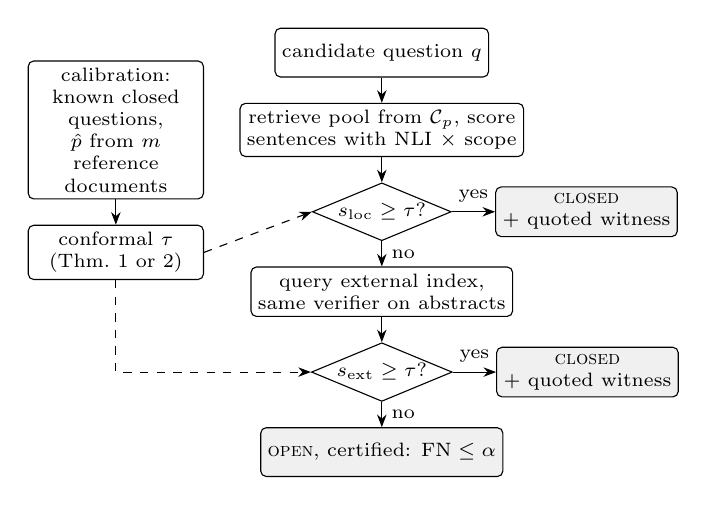
\begin{tikzpicture}[node distance=0.32cm, font=\scriptsize,
  box/.style={draw, rounded corners=2pt, align=center, minimum height=0.62cm, inner sep=2.5pt},
  dec/.style={draw, diamond, aspect=2.4, align=center, inner sep=0.5pt},
  arr/.style={-{Stealth[length=1.6mm]}}]
\node[box] (q) {candidate question $q$};
\node[box, below=of q] (loc) {retrieve pool from $\mathcal{C}_p$, score\\sentences with NLI $\times$ scope};
\node[dec, below=of loc] (d1) {$s_{\mathrm{loc}}\ge\tau$?};
\node[box, right=0.55cm of d1, fill=black!6] (c1) {\closed{}\\+ quoted witness};
\node[box, below=of d1] (ext) {query external index,\\same verifier on abstracts};
\node[dec, below=of ext] (d2) {$s_{\mathrm{ext}}\ge\tau$?};
\node[box, right=0.55cm of d2, fill=black!6] (c2) {\closed{}\\+ quoted witness};
\node[box, below=of d2, fill=black!6] (o) {\open{}, certified: $\mathrm{FN}\le\alpha$};
\node[box, left=0.45cm of loc, text width=2.05cm] (cal) {calibration:\\known closed questions,\\$\hat p$ from $m$ reference\\documents};
\node[box, below=of cal, text width=2.05cm] (tau) {conformal $\tau$\\(Thm.~1 or 2)};
\draw[arr] (q) -- (loc); \draw[arr] (loc) -- (d1);
\draw[arr] (d1) -- node[above]{yes} (c1); \draw[arr] (d1) -- node[right]{no} (ext);
\draw[arr] (ext) -- (d2); \draw[arr] (d2) -- node[above]{yes} (c2); \draw[arr] (d2) -- node[right]{no} (o);
\draw[arr] (cal) -- (tau);
\draw[arr, dashed] (tau.east) -- (d1.west);
\draw[arr, dashed] (tau.south) |- (d2.west);
\end{tikzpicture}
\caption{Certified gap declaration. Shaded boxes are outputs. The threshold $\tau$ is calibrated once and shared by both checks, so the combined score $\max\{s_{\mathrm{loc}},s_{\mathrm{ext}}\}$ is compared with a single $\tau$.}
\label{fig:pipe}
\end{figure}

\subsection{Evidence-scope verification (ESV-Scope)}
For each question we retrieve a pool of $K=10$ abstracts by reciprocal rank fusion~\cite{cormack2009} of BM25~\cite{robertson2009} and a MiniLM bi-encoder~\cite{reimers2019,wang2020minilm}. Every sentence $x$ of every pooled abstract $d$ is scored by an NLI cross-encoder, DeBERTa-v3-large~\cite{he2023debertav3} fine-tuned on MNLI, FEVER-NLI, ANLI, LingNLI and WANLI~\cite{laurer2024}, with the sentence as premise and the question as hypothesis. Let $e(x)$ and $c(x)$ be the entailment and contradiction probabilities. A sentence counts as a witness only if it is about the same question, so we multiply by a scope factor
\begin{equation}
\sigma(q,x,d)=\frac{|T(q)\cap(T(x)\cup T(t_d))|}{|T(q)|}\cdot \mathbf{1}[N(q)\subseteq N(d)],
\end{equation}
where $T(\cdot)$ is the set of stemmed content terms, $t_d$ the title of $d$, and $N(\cdot)$ the set of numbers. Facet coverage is computed on one sentence and its own title, never pooled across documents, so two half-relevant papers cannot combine into one false witness. The score is
\begin{equation}
s_{\mathrm{ESV}}(q;\mathcal{K})=\max_{d\in\mathcal{K}\cap P(q)}\ \max_{x\in d}\ \max\{e(x),c(x)\}\,\sigma(q,x,d)^{a},
\end{equation}
with $P(q)$ the retrieval pool and $a$ an exponent. The maximizing sentence is returned as the quoted witness. Because $s_{\mathrm{ESV}}$ is a maximum over available documents, it is monotone. For uncertified classification we also report ESV-Learned, a logistic head over eight verifier and scope features of the top three documents. It is more accurate but not monotone, so we do not use it for certification. We checked monotonicity empirically on the 809 training questions under two nested random deletion sets. CoMention, BM25, Dense and ESV-Scope over the full pool never increased, while NLI verification over the top five documents increased for 18 questions, ESV-Scope over the top five for 15 and ESV-Learned for 46.

\subsection{Certified \open{} decisions}
Let $S_1,\dots,S_n$ be scores of calibration questions known to be \closed{}, sorted increasingly, and let $k=\lfloor\alpha(n+1)\rfloor$. We set $\tau=S_{(k)}$ (and $\tau=-\infty$ if $k=0$) and declare \open{} iff $s<\tau$.

\begin{theorem}[In-situ calibration]
Suppose the calibration questions are scored against the same incomplete corpus $\mathcal{C}_p$ as the test question, their labels come from outside $\mathcal{C}_p$, and calibration and test questions are exchangeable. Then $\mathrm{FN}\le\alpha$ for every, possibly unknown, $p$.
\end{theorem}
\begin{proof}
The deletion mechanism does not depend on question identity, so the scores of the $n$ calibration questions and the test question are exchangeable. The rank of the test score is uniform among $n+1$ positions, hence $P(S_{\mathrm{test}}<S_{(k)})\le k/(n+1)\le\alpha$.
\end{proof}

Theorem~1 needs closed questions whose status is known independently of the local corpus, for example questions answered by papers cited in a recent review. Often the only labeled questions come from a curated, complete benchmark. The next result covers that case.

\begin{theorem}[Transfer calibration]
Assume that the calibration questions and the test question are exchangeable before any deletion, that the calibration scores are computed on a complete benchmark after deleting each of its witnesses independently with probability $\hat p$, and that the target corpus $\mathcal{C}_p$ follows the incompleteness model with $p\le\hat p$. If $s$ is monotone, then $\mathrm{FN}\le\alpha$ on $\mathcal{C}_p$.
\end{theorem}
\begin{proof}
Couple the corpora. Delete each witness with probability $p$ to obtain $\mathcal{C}_p$, then delete each surviving witness with probability $(\hat p-p)/(1-p)$. The result has the law of $\mathcal{C}_{\hat p}$ and satisfies $\mathcal{C}_{\hat p}\subseteq\mathcal{C}_p$. Monotonicity gives $s(q;\mathcal{C}_{\hat p})\le s(q;\mathcal{C}_p)$, so $P(s(q;\mathcal{C}_p)<\tau)\le P(s(q;\mathcal{C}_{\hat p})<\tau)$. At rate $\hat p$ the test score and the calibration scores are produced by the same deletion process from exchangeable questions, so they are exchangeable and the last probability is at most $\alpha$ as in Theorem~1.
\end{proof}

Both results rest on exchangeability. If the calibration questions come from a different population than the questions being screened, the bound can fail even with the correct $\hat p$. Section~VI measures how much this matters when calibrating on one SciFact split and testing on the other.

\begin{corollary}[Estimated coverage]
Sample $m$ witness documents of known closed questions uniformly, observe that $x$ of them are missing from $\mathcal{C}_p$, and let $\hat p$ be the one-sided $(1-\delta)$ Clopper-Pearson upper bound~\cite{clopper1934} for $x/m$. Then $\mathrm{FN}\le\alpha+\delta$.
\end{corollary}

Setting $\hat p=1$ needs no knowledge of coverage but places $\tau$ below the scores of closed questions whose witnesses are all missing. We call the resulting loss of power the \emph{price of certainty}.

\subsection{Targeted external evidence recovery}
Power is lost on closed questions that look open because their evidence is missing. The only remedy is to find that evidence elsewhere. For a question whose local score is below $\tau$, we query OpenAlex~\cite{priem2022}, keep the top ten works that have abstracts, and apply the same verifier and scope factor to their sentences. The final score is $\max\{s(q;\mathcal{C}_p), s_{\mathrm{ext}}(q)\}$. The external term does not depend on which local documents are missing, so the combined score stays monotone and both theorems still apply. External queries are needed only for questions that would otherwise be declared \open{}.

\section{Experimental Setup}
\textbf{Benchmark.} SciFact contains expert-written biomedical claims, a corpus of 5,183 abstracts, and rationale sentences~\cite{wadden2020}. We read every claim $q$ as the question ``is there published evidence on whether $q$?''. A claim with at least one \textsc{support} or \textsc{contradict} rationale is \closed{}, and its rationale documents are witnesses. A claim labeled \textsc{nei} is \open{} with respect to the corpus. SciFact claims are specific findings rather than the broader gap statements found in review articles, so GapClose-SciFact is a controlled surrogate for gap closure: it has expert evidence labels, which real gap lists lack, and it lets us delete evidence in a known way. Every \open{} claim has cited documents that are topically related but contain no evidence, which are exactly the documents that make co-mention heuristics fail. The SciFact training split (809 questions, 505 closed) is used for development and the development split (300 questions, 188 closed) for testing, since the official test labels are not public. The mapping was fixed before any system was run. Table~\ref{tab:bench} gives the statistics.

\begin{table}[t]
\centering
\caption{GapClose-SciFact statistics. Hard negatives are cited documents of \open{} questions that contain no evidence.}
\label{tab:bench}
\begin{tabular}{lcc}
\toprule
 & Train (dev.) & Test \\
\midrule
Questions & 809 & 300 \\
\quad \closed{} (support / contradict) & 505 (332 / 173) & 188 (124 / 64) \\
\quad \open{} (\textsc{nei}) & 304 & 112 \\
Witness documents & 564 & 209 \\
Hard-negative documents of \open{} & 330 & 114 \\
Corpus abstracts & \multicolumn{2}{c}{5,183} \\
\bottomrule
\end{tabular}
\end{table}

\textbf{Methods.} \emph{CoMention} scores a question by the largest fraction of its content terms that co-occur in one abstract, which mimics graph-link gap finders. \emph{BM25} and \emph{Dense} use the top retrieval score. \emph{BGE-large dense} uses the top cosine similarity of BGE-large-en-v1.5 embeddings, and \emph{BGE reranker} the highest cross-encoder relevance (bge-reranker-base) over the retrieval pool; these stand for the retrieval components of current RAG-based assistants. \emph{NLI-verify} takes the maximum non-neutral NLI probability over pooled sentences, without scope. \emph{ESV-Scope} and \emph{ESV-Learned} are described above. All models run through ONNX Runtime with the published weights.

\textbf{Protocol.} Every design choice of ESV (exponent $a\in\{0,0.25,0.5,1\}$, depth $k\in\{3,5,10\}$, scope-only versus learned head) was selected by five-fold cross-validation on the training split. We report two passes over the test split. A first pass used a smaller verifier (DeBERTa-v3-small) and untuned defaults, where ESV-Scope reached macro-F1 0.648 against 0.669 for CoMention. The second pass, reported below, used the large verifier and the configuration chosen by cross-validation. Certification is evaluated under two protocols, each with 500 repetitions. \emph{Resampled}: both splits are pooled and randomly halved into calibration and test questions, which matches the exchangeability assumption of the theorems. \emph{Train$\to$test}: calibration questions are a random half of the training split and the evaluation set is the whole test split, which was never used for choosing the certified scores. In every repetition a fresh global deletion pattern removes witness documents at rate $p\in\{0,0.1,0.2,0.3,0.5,0.7,1\}$, either independently (\emph{random}) or with probability proportional to the witness's ESV score (\emph{targeted}), so that strong evidence is missing more often than weak evidence. The targeted pattern violates the independent witness-deletion model on purpose. We use $\alpha=0.1$, $\delta=0.05$ and $m=100$ reference documents sampled uniformly from calibration witnesses. Certification uses the \Nquestions{} questions for which external results were available.

\section{Results}
\subsection{Accuracy without certification}
Table~\ref{tab:cls} shows the usual view. The strongest uncertified scores come from modern retrieval models. The BGE reranker reaches macro-F1 0.713 and the lowest AURC, ahead of ESV-Learned at 0.687. These models rank documents but quote no evidence, so a user cannot check why a question was called answered. Among methods that return a witness sentence, ESV-Learned is the most accurate and has the most precise witnesses: 58\% of its quoted sentences match a gold rationale, against 29\% for CoMention. Since a non-gold sentence can still be valid evidence, these figures are lower bounds on witness quality. Cross-validation on the training split explains the design (Table~\ref{tab:abl}). Without the scope factor ($a=0$) accuracy falls as more documents are verified, because every extra abstract adds chances for an off-topic sentence to look like entailment or contradiction. With scope, deeper verification no longer hurts, and the best scope-only setting improves on the best unscoped one by 0.053. The learned head adds another 0.014.

\begin{table}[t]
\centering
\caption{Five-fold cross-validated macro-F1 on the training split. Rows: scope exponent $a$ ($a=0$ is NLI without scope). Columns: number of verified documents $k$.}
\label{tab:abl}
\begin{tabular}{lccc}
\toprule
 & $k=3$ & $k=5$ & $k=10$ \\
\midrule
$a=0$ (no scope) & 0.651 & 0.631 & 0.615 \\
$a=0.25$ & 0.685 & 0.687 & 0.682 \\
$a=0.5$ & 0.694 & 0.682 & 0.696 \\
$a=1$ & 0.684 & 0.685 & \textbf{0.704} \\
ESV-Learned & \textbf{0.718} & 0.704 & 0.698 \\
\midrule
\multicolumn{4}{l}{Baselines: CoMention 0.660, Dense 0.654, BM25 0.643} \\
\bottomrule
\end{tabular}
\end{table} On 300 test questions the bootstrap intervals of all methods overlap, and none of the paired differences between ESV-Learned and the other methods is significant. The more serious problem is the false novelty column. Every method calls between 20\% and 32\% of answered questions open on a corpus that contains their evidence.

\begin{table}[t]
\centering
\caption{Uncertified gap-closure decisions on the SciFact test split (300 questions). FN: false novelty, FC: false closure, Wit.: share of quoted sentences that are gold rationales.}
\label{tab:cls}
\setlength{\tabcolsep}{3pt}
\begin{tabular}{lcccccc}
\toprule
Method & F1 & 95\% CI & FN & FC & Wit. & AURC \\
\midrule
CoMention & 0.669 & [0.61, 0.72] & 0.197 & 0.473 & 0.291 & 0.190 \\
BM25 & 0.660 & [0.60, 0.72] & 0.197 & 0.491 & n/a & 0.217 \\
Dense (MiniLM) & 0.631 & [0.58, 0.68] & 0.319 & 0.411 & n/a & 0.246 \\
BGE-large dense & 0.699 & [0.64, 0.75] & 0.213 & 0.393 & n/a & 0.185 \\
BGE reranker & \textbf{0.713} & [0.66, 0.77] & 0.245 & 0.321 & n/a & \textbf{0.124} \\
NLI-verify & 0.663 & [0.60, 0.71] & 0.239 & 0.438 & 0.503 & 0.225 \\
ESV-Learned & 0.687 & [0.63, 0.74] & 0.234 & 0.393 & 0.576 & 0.156 \\
\bottomrule
\end{tabular}

\end{table}

\subsection{Absence of evidence carries no signal}
If an incomplete corpus still held traces of a missing answer, a better local score could fix false novelty. We tested this directly. On the training split we deleted all witness documents and measured how well signals that survive the deletion separate the 505 closed questions from the 304 open ones (Table~\ref{tab:auc}). They include the two strongest uncertified scores of Table~\ref{tab:cls}, the density of related literature, the verifier score on the remaining documents, the proportion of neutral NLI judgments, sentences that state uncertainty (``remains unclear'', ``no studies have examined''), and properties of the question itself. All AUC values lie between 0.45 and 0.55. For the signals we tested, an answered question whose evidence is gone looks the same as an unanswered one. We cannot rule out that some other local feature carries information, but the Proposition in Section~III shows that no local rule can be certified without an assumption on coverage, and Table~\ref{tab:auc} suggests that in practice the local signals do not even help as heuristics.

\begin{table}[t]
\centering
\caption{Separating closed from open questions after all witnesses are deleted (training split, 505 vs.\ 304). 0.5 is chance.}
\label{tab:auc}
\begin{tabular}{lc}
\toprule
Signal available after deletion & AUC \\
\midrule
Dense similarity, top-1 / mean of top-5 & 0.517 / 0.546 \\
BGE-large dense, top-1 & 0.496 \\
BGE reranker, best pooled document & 0.502 \\
BM25 score, top-1 & 0.488 \\
ESV-Scope on remaining documents & 0.529 \\
Mean neutral NLI probability & 0.508 \\
Uncertainty cue sentences, count / scoped & 0.495 / 0.537 \\
Question length / has number / negation & 0.485 / 0.451 / 0.489 \\
\bottomrule
\end{tabular}
\end{table}

\subsection{Certification under incompleteness}
Fig.~\ref{fig:cert} and Table~\ref{tab:fn} report false novelty as evidence is removed. The F1-optimal threshold, which is what a tuned gap finder would use, starts at \FNfoneZero{} and climbs to \FNfoneOne{} when all evidence is missing. The most accurate uncertified score, the BGE reranker, goes from \FNbgeZero{} to \FNbgeOne{}: a better ranker makes a tuned threshold more confident, and therefore more often wrong, once the evidence is gone. Standard split-conformal calibration on the complete corpus meets the 10\% target at $p=0$, as theory predicts, but exceeds it from $p=0.1$ on and reaches \FNconfOne{}. The same happens for \NconfViolOne{} of the \Nscores{} scores at $p=0.1$ and for all of them by $p=\ConfAllBy{}$. A guarantee proved for a complete corpus does not survive the realistic case. In-situ calibration (Theorem~1) and transfer calibration with the estimated $\hat p$ (Theorem~2 and the corollary) stay at the target at every incompleteness rate and for all \Nscores{} scores we evaluated. The largest mean over 500 splits is \MaxInsitu{} for in-situ and \MaxTransfer{} for transfer calibration, which is within Monte Carlo error of 0.10. The estimate is conservative but close. For $p=0.3$ its mean is \phatThree{}, from only 100 sampled reference documents.

Table~\ref{tab:robust} stresses the two assumptions. Under resampling, targeted deletion barely moves the certified rules (largest mean \RobPTAllTr{} over all scores), even though the independent witness-deletion model no longer holds, while split conformal fails as before. Calibrating on the training split and testing on the fixed test split gives higher values. For ESV-Scope the transfer rule stays at \RobHMEsvTr{} and the in-situ rule reaches \RobHMEsvIn{}, while the largest value over all scores and rates is \RobHMAllTr{}. These numbers must be read with care. The test split contains only \NholdClosed{} closed questions, so a false-novelty rate measured on it has a binomial standard error of about \SEhold{} even when the guarantee holds, and the largest of 70 correlated estimates is biased upward. The excess is also present at $p=0$, where nothing is deleted. We therefore cannot separate a shift between the two SciFact splits from sampling noise, but the experiment shows that a guarantee calibrated on one population should not be read as exact on another. Calibration questions should be drawn from the same field and the same type of question as the candidates being screened.

\begin{table}[t]
\centering
\caption{Largest mean false novelty over all deletion rates (target 0.10). ``All scores'' takes the maximum over every certified score. Values above 0.105 in bold.}
\label{tab:robust}
\setlength{\tabcolsep}{2.5pt}
\begin{tabular}{lccccc}
\toprule
 & \multicolumn{2}{c}{ESV-Scope} & \multicolumn{2}{c}{All scores} & Split conf. \\
\cmidrule(lr){2-3}\cmidrule(lr){4-5}\cmidrule(lr){6-6}
Evaluation setting & in-situ & transfer & in-situ & transfer & ESV-Scope \\
\midrule
Resampled, random deletion & 0.099 & 0.094 & 0.101 & 0.100 & \textbf{0.302} \\
Resampled, targeted deletion & 0.099 & 0.094 & 0.101 & 0.104 & \textbf{0.277} \\
Train$\to$test, random deletion & \textbf{0.117} & 0.104 & \textbf{0.126} & \textbf{0.126} & \textbf{0.299} \\
Train$\to$test, targeted deletion & \textbf{0.115} & \textbf{0.108} & \textbf{0.125} & \textbf{0.125} & \textbf{0.279} \\
\bottomrule
\end{tabular}

\end{table}

\begin{table}[t]
\centering
\caption{Mean false novelty of ESV-Scope over 500 random splits, target $\alpha=0.10$. Values above the target are in bold.}
\label{tab:fn}
\setlength{\tabcolsep}{3pt}
\begin{tabular}{lccccc}
\toprule
Rule & $p=0$ & $p=0.1$ & $p=0.3$ & $p=0.5$ & $p=1$ \\
\midrule
F1-optimal threshold & \textbf{0.309} & \textbf{0.343} & \textbf{0.415} & \textbf{0.489} & \textbf{0.672} \\
Split conformal (complete) & 0.099 & \textbf{0.117} & \textbf{0.153} & \textbf{0.196} & \textbf{0.302} \\
In-situ conformal (Thm.~1) & 0.099 & 0.098 & 0.098 & 0.098 & 0.071 \\
Transfer, $\hat p$ (Thm.~2) & 0.094 & 0.089 & 0.087 & 0.090 & 0.071 \\
Transfer, $\hat p=1$ & 0.012 & 0.016 & 0.030 & 0.037 & 0.071 \\
\bottomrule
\end{tabular}

\end{table}

\begin{figure*}[t]
\centering
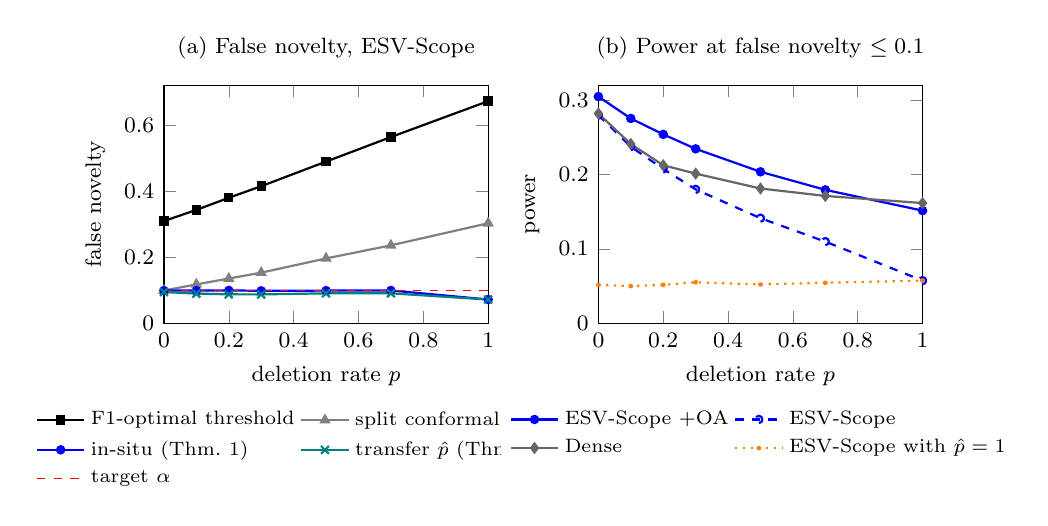
\begin{tikzpicture}
\begin{axis}[name=left, width=0.47\textwidth, height=4.6cm, xmin=0, xmax=1, ymin=0, ymax=0.72,
  xlabel={deletion rate $p$}, ylabel={false novelty}, label style={font=\footnotesize},
  tick label style={font=\footnotesize}, title={(a) False novelty, ESV-Scope}, title style={font=\footnotesize},
  legend style={font=\scriptsize, at={(0.5,-0.32)}, anchor=north, legend columns=2, draw=none},
  legend cell align=left]
\addplot[thick, black, mark=square*, mark size=1.3pt] coordinates {(0,0.3092) (0.1,0.3429) (0.2,0.3796) (0.3,0.4147) (0.5,0.4892) (0.7,0.5636) (1,0.6723)};
\addplot[thick, gray, mark=triangle*, mark size=1.6pt] coordinates {(0,0.0987) (0.1,0.1172) (0.2,0.1350) (0.3,0.1528) (0.5,0.1959) (0.7,0.2355) (1,0.3024)};
\addplot[thick, blue, mark=*, mark size=1.3pt] coordinates {(0,0.0987) (0.1,0.0984) (0.2,0.0990) (0.3,0.0978) (0.5,0.0984) (0.7,0.0989) (1,0.0714)};
\addplot[thick, teal, mark=x, mark size=2pt] coordinates {(0,0.0940) (0.1,0.0894) (0.2,0.0871) (0.3,0.0869) (0.5,0.0901) (0.7,0.0902) (1,0.0714)};
\addplot[dashed, red, domain=0:1, samples=2] {0.1};
\legend{F1-optimal threshold, split conformal (complete), in-situ (Thm.~1), transfer $\hat p$ (Thm.~2), target $\alpha$}
\end{axis}
\begin{axis}[at={(left.east)}, anchor=west, xshift=1.4cm, width=0.47\textwidth, height=4.6cm, xmin=0, xmax=1, ymin=0, ymax=0.32,
  xlabel={deletion rate $p$}, ylabel={power}, label style={font=\footnotesize},
  tick label style={font=\footnotesize}, title={(b) Power at false novelty $\le 0.1$}, title style={font=\footnotesize},
  legend style={font=\scriptsize, at={(0.5,-0.32)}, anchor=north, legend columns=2, draw=none},
  legend cell align=left]
\addplot[thick, blue, mark=*, mark size=1.3pt] coordinates {(0,0.3050) (0.1,0.2755) (0.2,0.2541) (0.3,0.2346) (0.5,0.2037) (0.7,0.1794) (1,0.1514)};
\addplot[thick, blue, dashed, mark=o, mark size=1.3pt] coordinates {(0,0.2799) (0.1,0.2376) (0.2,0.2075) (0.3,0.1800) (0.5,0.1412) (0.7,0.1097) (1,0.0572)};
\addplot[thick, black!60, mark=diamond*, mark size=1.6pt] coordinates {(0,0.2821) (0.1,0.2411) (0.2,0.2125) (0.3,0.2013) (0.5,0.1812) (0.7,0.1712) (1,0.1616)};
\addplot[thick, orange, dotted, mark=star, mark size=1.6pt] coordinates {(0,0.0516) (0.1,0.0499) (0.2,0.0515) (0.3,0.0550) (0.5,0.0520) (0.7,0.0543) (1,0.0572)};
\legend{ESV-Scope +OA, ESV-Scope, Dense, ESV-Scope with $\hat p=1$}
\end{axis}
\end{tikzpicture}

\caption{(a) False novelty of ESV-Scope as witness documents are deleted, mean over 500 random splits. Only the certified rules stay at the target $\alpha=0.1$ (dashed). (b) Power of certified rules with transfer calibration, and the worst-case rule $\hat p=1$ for comparison.}
\label{fig:cert}
\end{figure*}

The guarantee has a cost, shown in Table~\ref{tab:power}. With transfer calibration ESV-Scope certifies \PowESVZero{} of truly open questions on a complete corpus and \PowESVHalf{} at $p=0.5$. Without any estimate of coverage ($\hat p=1$) power falls to \PowESVWorst{}. A stronger ranker turns directly into more certified gaps. The BGE reranker certifies \PowBGEZero{} of open questions on a complete corpus, but its advantage shrinks to \PowBGEHalf{} at $p=0.5$ and \PowBGEOne{} at $p=1$, because no ranking quality can recover documents that are not there. Estimating coverage from a small reference sample therefore pays for itself. It certifies 4.8, 3.3 and 2.7 times as many gaps as the worst-case rule at $p=0.1$, $0.3$ and $0.5$.

\subsection{External recovery}
Table~\ref{tab:power} also shows the effect of querying OpenAlex for low-scoring questions. On its own the external score separates closed from open questions only moderately (AUC 0.633 on the training split and 0.581 on the test split), and it found the exact SciFact witness for only 14\% of closed questions. It still helps where it matters. With ESV-Scope plus external evidence, power at $p=0.5$ rises from \PowESVHalf{} to \PowOAHalf{} and the worst-case power nearly triples, from \PowESVWorst{} to \PowOAWorst{}. The same search cuts the false novelty of the F1-optimal threshold at $p=1$ from \FNfoneOne{} to \FNfoneOAOne{}. External queries were issued for \ExtCalls{} of questions at $p=0.5$. Search also helps the strongest ranker: the BGE reranker with external evidence has the highest power at moderate incompleteness (0.266 at $p=0.3$ and 0.214 at $p=0.5$), so the two ingredients, a good closure score and evidence from outside the corpus, add up. At high incompleteness the plain Dense score remains competitive, because similarity to the remaining literature is a weak but monotone hint that a field has been studied.

\begin{table}[t]
\centering
\caption{Power (share of truly open questions certified) at false novelty $\le 0.10$. ``+OA'': with targeted OpenAlex evidence. Worst case uses $\hat p=1$.}
\label{tab:power}
\setlength{\tabcolsep}{3pt}
\begin{tabular}{lccccc}
\toprule
 & \multicolumn{4}{c}{Transfer, estimated $\hat p$} & Worst case \\
\cmidrule(lr){2-5}
Score & $p=0$ & $p=0.3$ & $p=0.5$ & $p=1$ & any $p$ \\
\midrule
CoMention & 0.300 & 0.184 & 0.143 & 0.114 & 0.114 \\
Dense & 0.282 & 0.201 & 0.181 & \textbf{0.162} & \textbf{0.162} \\
BGE-large dense & 0.397 & 0.229 & 0.174 & 0.102 & 0.102 \\
BGE reranker & \textbf{0.443} & 0.235 & 0.173 & 0.097 & 0.097 \\
NLI-verify & 0.249 & 0.149 & 0.122 & 0.081 & 0.081 \\
ESV-Scope & 0.280 & 0.180 & 0.141 & 0.057 & 0.052 \\
\midrule
CoMention +OA & 0.288 & 0.210 & 0.161 & 0.115 & 0.115 \\
Dense +OA & 0.299 & 0.209 & 0.171 & 0.143 & 0.144 \\
BGE reranker +OA & 0.440 & \textbf{0.266} & \textbf{0.214} & 0.145 & 0.146 \\
ESV-Scope +OA & 0.305 & 0.235 & 0.204 & 0.151 & 0.150 \\
\bottomrule
\end{tabular}

\end{table}

\begin{table*}[t]
\centering
\caption{Examples from the test split and from external search. Witness sentences are quoted from the retrieved abstracts.}
\label{tab:ex}
\small
\begin{tabular}{>{\raggedright\arraybackslash}p{4.3cm}>{\raggedright\arraybackslash}p{1.3cm}>{\raggedright\arraybackslash}p{8.2cm}>{\raggedright\arraybackslash}p{2.2cm}}
\toprule
Question (claim) & Gold & Highest-scoring sentence & Decision \\
\midrule
PD-1 triggering on monocytes reduces IL-10 production by monocytes. & \closed{} & ``Triggering of PD-1 expressed on monocytes by PD-L1 \ldots{} induced IL-10 production'' (contradiction, local witness) & \closed{}, correct \\
Patients in stable partnerships have a faster progression from HIV to AIDS. & \closed{} & ``A stable partnership is associated with a slower rate of progression to AIDS or death'' (contradiction, local witness) & \closed{}, correct \\
Ethanol stress decreases the expression of IBP in bacteria. & \open{} & ``\ldots{} adaptation involves metabolic rewiring that boosts intracellular ethanol degradation'' (NLI 0.99, scope 0.16) & NLI alone: false closure; ESV: no witness \\
CCL19 is a ligand for CCR7. & \closed{} & ``The CCR7 ligands, CCL19 and CCL21, coordinate lymph node homing \ldots'' (entailment, external, not the SciFact witness) & \closed{} via OpenAlex \\
4-PBA treatment raises endoplasmic reticulum stress \ldots & \open{} (\textsc{nei}) & ``ER stress inhibition, via 4-PBA, blunted the development of hypertension'' (contradiction, external, 2017) & answered outside the corpus \\
\bottomrule
\end{tabular}
\end{table*}

\section{Discussion and Limitations}
\textbf{Examples.} Table~\ref{tab:ex} shows typical cases. The first two are contradictions that a gap finder relying on co-mention would also link, but only a sentence-level verifier can say that the literature answers the question in the opposite direction. The third shows why scope matters: an abstract about ethanol adaptation says little about the stated protein, yet unscoped NLI gives 0.99. The last two come from external search. One recovers a closure through a different paper from the SciFact witness, and the other answers a question that SciFact labels as lacking evidence.

\textbf{What a gap finder should report.} Our results suggest that a list of gaps without an error statement is not informative. The score with the best accuracy, the BGE reranker, also has the highest false novelty when evidence is missing (\FNbgeOne{} at $p=1$), because accuracy rewards a threshold that guesses \open{} whenever evidence is weak. A certified rule is more modest. It reports fewer gaps, states the false-novelty level it guarantees, and quotes the sentence that closes every question it declares \closed{}.

\textbf{Benchmark labels are corpus-relative.} \textsc{nei} in SciFact means that no evidence exists in 5,183 abstracts, not in the literature. Inspecting external evidence, we found \open{} questions that are in fact answered elsewhere. For example, the claim that 4-PBA raises endoplasmic reticulum stress is contradicted by a 2017 study that uses 4-PBA as an ER stress inhibitor. Such cases lower the measured power of methods with external search, so the external gains above are conservative. They also show that a widely used benchmark contains the very error we study.

\textbf{Using the method in practice.} A deployment needs two ingredients besides the verifier. The first is a set of closed questions with known answers in the target field, for example claims extracted from the included studies of recent systematic reviews, whose status does not depend on the local corpus. With them, Theorem~1 applies directly and no estimate of coverage is needed. The second, for transfer calibration, is a sample of evidence-bearing studies, for example the included studies that a recent systematic review cites as answering its questions, which gives $\hat p$ by a simple membership check. The Corollary needs these studies to be witnesses, not merely related papers: the missing rate of loosely related references need not bound the missing rate of evidence. One hundred references were enough in our experiments, and the Clopper-Pearson bound stayed conservative at every rate. Reporting should state $\alpha$, $\hat p$ and the number of calibration questions next to every list of gaps.

\textbf{Limitations.} Theorem~2 assumes independent witness deletion. Targeted deletion of strong evidence changed the certified error by less than half a point in our experiments, but real corpora can lose papers in other systematic ways, for example by year, language or access, and $\hat p$ should then be estimated within the relevant stratum. The larger risk is a shift between calibration and screened questions, which the theorems do not cover. Our held-out experiment (Table~\ref{tab:robust}) is too small to confirm or rule out such a shift, and weighted conformal methods~\cite{tibshirani2019} are a natural next step. GapClose-SciFact is a surrogate built from one biomedical benchmark, and its \open{} labels are corpus-relative. We did not evaluate language-model judges. The guarantee is model-agnostic, but we expect the same failure for any judge that sees only the local corpus, since the Proposition in Section~III applies to every such rule. The verifier could not be fine-tuned because our environment did not support PyTorch, so the learned component is a logistic head on frozen NLI outputs. The test split was evaluated twice for uncertified accuracy, as reported in Section~V. Finally, a question that is closed by our definition may still deserve new work, for instance in a different population or setting. Certification addresses false novelty at the level of the stated question, not research value.

\section{Conclusion}
A missing answer in a corpus is not evidence that a question is open. On GapClose-SciFact, accuracy-tuned rules declare up to 32\% of answered questions open on a complete corpus and up to 73\% when evidence is missing, standard conformal guarantees break for most scores once a tenth of the evidence is absent, and no local signal recovers the difference. Conformal calibration that accounts for incompleteness, in situ or with an estimated missing rate, keeps false novelty under the target at every tested rate when calibration questions are exchangeable with the screened ones, and targeted external search buys back part of the power that the guarantee costs. We release the benchmark, deletion protocol and code so that future gap-finding systems can report how often their gaps are false.

\begin{thebibliography}{99}
\bibitem{swanson1986} D. R. Swanson, ``Undiscovered public knowledge,'' \emph{The Library Quarterly}, vol. 56, no. 2, pp. 103-121, 1986.
\bibitem{baek2025} J. Baek, S. K. Jauhar, S. Cucerzan, and S. J. Hwang, ``ResearchAgent: Iterative research idea generation over scientific literature with large language models,'' in \emph{Proc. NAACL}, 2025.
\bibitem{wang2024scimon} Q. Wang, D. Downey, H. Ji, and T. Hope, ``SciMON: Scientific inspiration machines optimized for novelty,'' in \emph{Proc. ACL}, 2024.
\bibitem{si2025} C. Si, D. Yang, and T. Hashimoto, ``Can LLMs generate novel research ideas? A large-scale human study with 100+ NLP researchers,'' in \emph{Proc. ICLR}, 2025.
\bibitem{mullerbloch2015} C. M\"uller-Bloch and J. Kranz, ``A framework for rigorously identifying research gaps in qualitative literature reviews,'' in \emph{Proc. ICIS}, 2015.
\bibitem{wadden2020} D. Wadden, S. Lin, K. Lo, L. L. Wang, M. van Zuylen, A. Cohan, and H. Hajishirzi, ``Fact or fiction: Verifying scientific claims,'' in \emph{Proc. EMNLP}, 2020, pp. 7534-7550.
\bibitem{wadden2022multivers} D. Wadden, K. Lo, L. L. Wang, A. Cohan, I. Beltagy, and H. Hajishirzi, ``MultiVerS: Improving scientific claim verification with weak supervision and full-document context,'' in \emph{Findings of NAACL}, 2022.
\bibitem{wadden2022open} D. Wadden, K. Lo, B. Kuehl, A. Cohan, I. Beltagy, L. L. Wang, and H. Hajishirzi, ``SciFact-Open: Towards open-domain scientific claim verification,'' in \emph{Findings of EMNLP}, 2022.
\bibitem{thorne2018} J. Thorne, A. Vlachos, C. Christodoulopoulos, and A. Mittal, ``FEVER: A large-scale dataset for fact extraction and VERification,'' in \emph{Proc. NAACL}, 2018.
\bibitem{vovk2005} V. Vovk, A. Gammerman, and G. Shafer, \emph{Algorithmic Learning in a Random World}. New York: Springer, 2005.
\bibitem{lei2018} J. Lei, M. G'Sell, A. Rinaldo, R. J. Tibshirani, and L. Wasserman, ``Distribution-free predictive inference for regression,'' \emph{J. Amer. Statist. Assoc.}, vol. 113, no. 523, pp. 1094-1111, 2018.
\bibitem{angelopoulos2023} A. N. Angelopoulos and S. Bates, ``Conformal prediction: A gentle introduction,'' \emph{Found. Trends Mach. Learn.}, vol. 16, no. 4, pp. 494-591, 2023.
\bibitem{tibshirani2019} R. J. Tibshirani, R. Foygel Barber, E. Cand\`es, and A. Ramdas, ``Conformal prediction under covariate shift,'' in \emph{Proc. NeurIPS}, 2019.
\bibitem{barber2023} R. Foygel Barber, E. J. Cand\`es, A. Ramdas, and R. J. Tibshirani, ``Conformal prediction beyond exchangeability,'' \emph{Ann. Statist.}, vol. 51, no. 2, pp. 816-845, 2023.
\bibitem{angelopoulos2024crc} A. N. Angelopoulos, S. Bates, A. Fisch, L. Lei, and T. Schuster, ``Conformal risk control,'' in \emph{Proc. ICLR}, 2024.
\bibitem{geifman2017} Y. Geifman and R. El-Yaniv, ``Selective classification for deep neural networks,'' in \emph{Proc. NeurIPS}, 2017.
\bibitem{little2019} R. J. A. Little and D. B. Rubin, \emph{Statistical Analysis with Missing Data}, 3rd ed. Hoboken, NJ: Wiley, 2019.
\bibitem{cormack2009} G. V. Cormack, C. L. A. Clarke, and S. Buettcher, ``Reciprocal rank fusion outperforms Condorcet and individual rank learning methods,'' in \emph{Proc. SIGIR}, 2009, pp. 758-759.
\bibitem{robertson2009} S. Robertson and H. Zaragoza, ``The probabilistic relevance framework: BM25 and beyond,'' \emph{Found. Trends Inf. Retr.}, vol. 3, no. 4, pp. 333-389, 2009.
\bibitem{reimers2019} N. Reimers and I. Gurevych, ``Sentence-BERT: Sentence embeddings using Siamese BERT-networks,'' in \emph{Proc. EMNLP-IJCNLP}, 2019.
\bibitem{wang2020minilm} W. Wang, F. Wei, L. Dong, H. Bao, N. Yang, and M. Zhou, ``MiniLM: Deep self-attention distillation for task-agnostic compression of pre-trained transformers,'' in \emph{Proc. NeurIPS}, 2020.
\bibitem{he2023debertav3} P. He, J. Gao, and W. Chen, ``DeBERTaV3: Improving DeBERTa using ELECTRA-style pre-training with gradient-disentangled embedding sharing,'' in \emph{Proc. ICLR}, 2023.
\bibitem{laurer2024} M. Laurer, W. van Atteveldt, A. Casas, and K. Welbers, ``Less annotating, more classifying: Addressing the data scarcity issue of supervised machine learning with deep transfer learning and BERT-NLI,'' \emph{Political Analysis}, vol. 32, no. 1, pp. 84-100, 2024.
\bibitem{clopper1934} C. J. Clopper and E. S. Pearson, ``The use of confidence or fiducial limits illustrated in the case of the binomial,'' \emph{Biometrika}, vol. 26, no. 4, pp. 404-413, 1934.
\bibitem{priem2022} J. Priem, H. Piwowar, and R. Orr, ``OpenAlex: A fully-open index of scholarly works, authors, venues, institutions, and concepts,'' arXiv:2205.01833, 2022.
\end{thebibliography}

\end{document}
